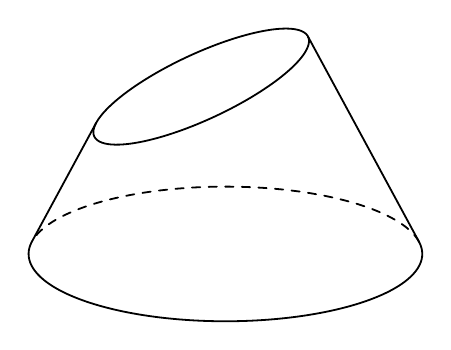
\begin{tikzpicture}[x=10mm,y=10mm,line width=.65pt,line cap=round,line join=round]
% Cone x^2+y^2=(H-z)^2/4, cut by z=2.4+.45x.
% Orthographic elevation 20 degrees; the cut is not parallel to the base.
\def\H{5}
\def\cut{2.4}
\def\slope{.45}
\def\elev{20}
\pgfmathsetmacro{\tangent}{asin(tan(\elev)/2)}
\pgfmathsetmacro{\other}{180-\tangent}
\pgfmathsetmacro{\rleft}{(\H-\cut)/(2+\slope*cos(\other))}
\pgfmathsetmacro{\rright}{(\H-\cut)/(2+\slope*cos(\tangent))}
\draw[dashed,domain=\tangent:\other,samples=80,smooth,variable=\t]
 plot ({2.5*cos(\t)},{2.5*sin(\elev)*sin(\t)});
\draw[domain=\other:360+\tangent,samples=80,smooth,variable=\t]
 plot ({2.5*cos(\t)},{2.5*sin(\elev)*sin(\t)});
\draw ({2.5*cos(\other)},{2.5*sin(\elev)*sin(\other)})--
 ({\rleft*cos(\other)},{sin(\elev)*\rleft*sin(\other)+cos(\elev)*(\H-2*\rleft)});
\draw ({2.5*cos(\tangent)},{2.5*sin(\elev)*sin(\tangent)})--
 ({\rright*cos(\tangent)},{sin(\elev)*\rright*sin(\tangent)+cos(\elev)*(\H-2*\rright)});
\draw[domain=0:360,samples=121,smooth,variable=\t]
 plot ({(\H-\cut)*cos(\t)/(2+\slope*cos(\t))},
 {sin(\elev)*(\H-\cut)*sin(\t)/(2+\slope*cos(\t))
 +cos(\elev)*(\H-2*(\H-\cut)/(2+\slope*cos(\t)))});
\end{tikzpicture}
